% Copyright (c) 2021 Robert Ryszard Paciorek <rrp@opcode.eu.org>
% 
% MIT License
% 
% Permission is hereby granted, free of charge, to any person obtaining a copy
% of this software and associated documentation files (the "Software"), to deal
% in the Software without restriction, including without limitation the rights
% to use, copy, modify, merge, publish, distribute, sublicense, and/or sell
% copies of the Software, and to permit persons to whom the Software is
% furnished to do so, subject to the following conditions:
% 
% The above copyright notice and this permission notice shall be included in all
% copies or substantial portions of the Software.
% 
% THE SOFTWARE IS PROVIDED "AS IS", WITHOUT WARRANTY OF ANY KIND, EXPRESS OR
% IMPLIED, INCLUDING BUT NOT LIMITED TO THE WARRANTIES OF MERCHANTABILITY,
% FITNESS FOR A PARTICULAR PURPOSE AND NONINFRINGEMENT. IN NO EVENT SHALL THE
% AUTHORS OR COPYRIGHT HOLDERS BE LIABLE FOR ANY CLAIM, DAMAGES OR OTHER
% LIABILITY, WHETHER IN AN ACTION OF CONTRACT, TORT OR OTHERWISE, ARISING FROM,
% OUT OF OR IN CONNECTION WITH THE SOFTWARE OR THE USE OR OTHER DEALINGS IN THE
% SOFTWARE.

\section{Realizacja instalacji elektrycznych}

Na instalację elektryczną składają się rozdzielnice wraz z zabezpieczeniami i innym osprzętem, okablowanie / oprzewodowanie (kable elektryczne, szynoprzewody), osprzęt elektroinstalacyjny (gniazdka, łączniki, ...).

\subsection{topologie}

Każda instalacja posiada pewną topologię, którą stanowi układ połączeń rozdzielnic i osprzętu oraz odbiorników przy pomocy okablowania / oprzewodowania.
Wyróżnić można kilka podstawowych topologi:
\begin{itemize}
	\item \strong{magistralę} – urządzenia dołączane są do przewodu przebiegającego przez nie, bądź w ich pobliżu (przy pomocy krótkich odgałęzień)
	%\begin{itemize}
		\item \strong{pierścień} – magistrala której końce są ze sobą połączone
	%\end{itemize}
	\item \strong{gwiazdę} – przewody od urządzeń zbiegają się w jednym punkcie i tam następują połączenia.
\end{itemize}
W praktyce na ogół spotyka się różnego rodzaju układy mieszane takie jak:
\begin{itemize}
	\item gwiazda magistral / pierścieni – np. z rozdzielnicy wychodzą 3 magistrale /pierścienie do których przyłączone są kolejne gniazdka
	\item magistrala gwiazd – np. na szynoprzewodzie (stanowiącym magistralę) zamontowane są skrzynki odpływowe z których wychodzą obwody do zasilania odbiorników (w układzie gwiazdy)
	\item gwiazda wielokrotna - np. z głównej rozdzielnicy wychodzi 5 obwodów, każdy przeznaczony do zasilania kolejnej rozdzielnicy
\end{itemize}\nopagebreak[4]%
i ich kombinacje.\pagebreak[1]

Układ z rozdzielnią główną oraz podrozdzielnicami umieszczonymi na obiekcie jest bardzo popularny w przemyśle i obiektach komercyjnych (biura, hotele, obiekty handlowe, itd.), natomiast (co trochę dziwne) nie jest sotowany nawet w dużych domach jednorodzinnych (gdzie pojedyncza rozdzielnica potrafi przekraczać 400 modułów).

Zaletą magistral jest mniejsza ilość przewodu potrzebnego do ich wykonania oraz mniejsza ilość obwodów pojawiających się w rozdzielnicy.
Zaletą gwiazdy jest możliwość sterowania dowolnym z obwodów z punktu centralnego (rozdzielnicy) i stosunkowo łatwej rekonfiguracji
	(np. podzielenia obwodu gniazd złożonego z kilku/kilkunastu przewodów wprowadzonych do rozdzielni zakończonych gniazdami, a podłączonych do jednego zabezpieczenia na kilka niezależnych obwodów podłączonych do osobnych zabezpieczeń).
Często też stosowane są rozwiązania pośrednie czyli (ze względu na sterowanie – \textit{inteligentny budynek} okablowanie wykonywane jest w gwiazdę,
	ale nie dotyczy to każdego gniazdka (bo nie planujemy sterowania nimi) i do rozdzielni trafiają przewody od grup gniazdek łączonych magistralą (np. 1 lub 2 grupy na pomieszczenie).

Oczywiście możliwe jest też wykonanie sterowania w układzie nie będącym gwiazdą (czyli np. sterowania indywidualnego każdym gniazdkiem w grupie spiętej na jednej magistrali) – wymaga to zastosowania rozproszonych modułów sterujących (np. zlokalizowanych w każdym z gniazdek).

\subsection{trasy kablowe}

Instalacje elektryczne mogą być prowadzone/montowane na dwa sposoby:
\begin{itemize}
	\item po wierzchu
	\item ukryte w ścianach, podłogach, itd (instalacje „podtynkowe”)
\end{itemize}

Zasadniczymi różnicami pomiędzy tymi sposobami prowadzenia instalacji jest łatwość ich prowadzenia i późniejszej modyfikacji vs względy estetyczne.
Przy czym warto tutaj zaznaczyć iż ładnie wykonana imnstalacja „natynkowa” jest estetyczna i dla niektórych stylów urządzania wnętrz może być wręcz atutem.

Instalacje prowadzone po wierzchu dominują w zastosowaniach przemysłowych, natomiast te ukryte w mieszkaniowych.
Funkcjonują także rozwiązania „kompromisowe”, często spotykane w obiektach komercyjnych (biura, obiekty handlowe, starsze rozwiązania serwerowni\footnote{Obecnie serwerownie realizowane są coraz częściej „po wierzchu”, jak typowy przemysł.}
	– ukrycie instalacji nad sufitami kasetonowymi, pod podłogami podnoszonymi, zastosowanie plastikowych kanałów instalacyjnych na których bezpośrednio montowany jest osprzęt elektryczny.

Pośród instalacji prowadzonych na wierzchu można wyróżnić kilka sposobów ich prowadzenia (mogą być one też mieszane w ramach danej instalacji):
\begin{itemize}
	\item szynoprzewody
	\item koryta metalowe (pełne, perforowane lub siatkowe) i drabiny kablowe
	\item rurki plastikowe
	\item przewód montowany bezpośrednio na uchwytach kablowych
	\item plastikowe korytka i kanały instalacyjne
\end{itemize}

Należy zachować odległość pomiędzy trasami w których prowadzone jest wysokoprądowe okablowanie zasilające od tras w których prowadzone jest „miedziane” (nie światłowodowe) okablowanie sterujące, telekomunikacyjne lub inne okablowanie „niskoprądowe”.

\begin{figure}[ht!]
\begin{center}\begin{tabular}{cc}
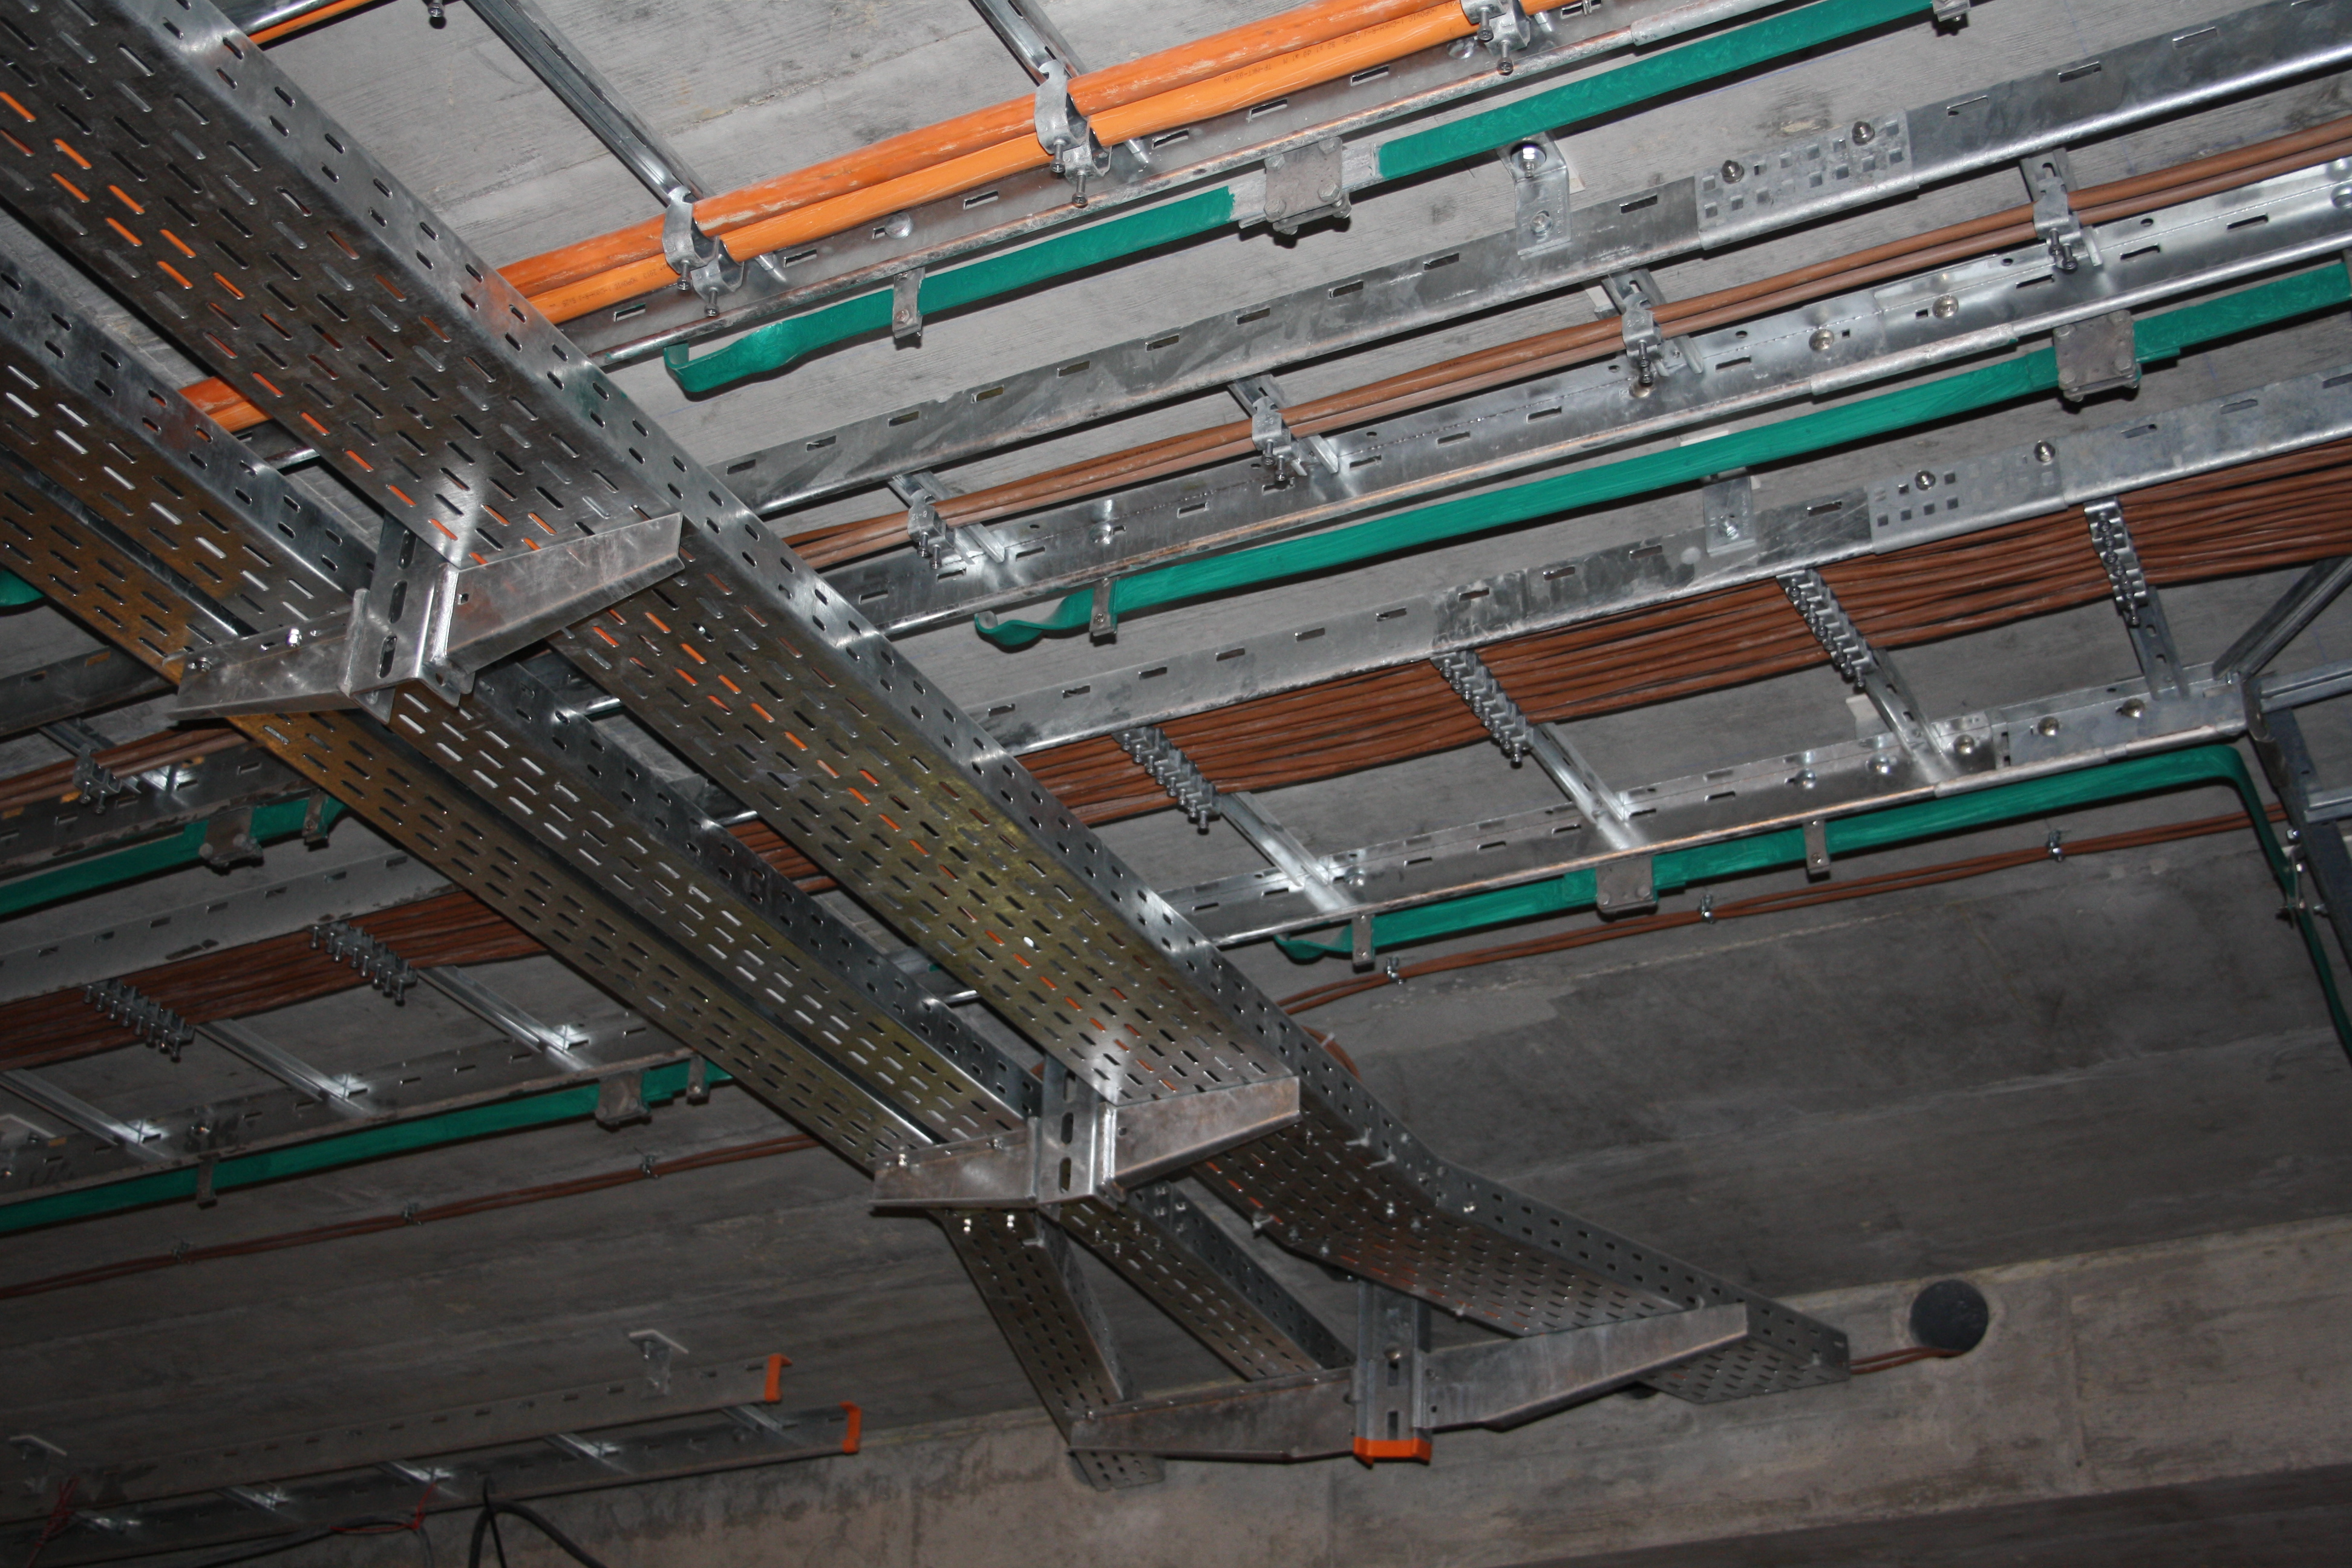
\includegraphics[width=0.47\textwidth]{elektryka/Cabtray_11.jpg} & % https://commons.wikimedia.org/wiki/File:Cabtray_11.jpg  Leotard, CC-0
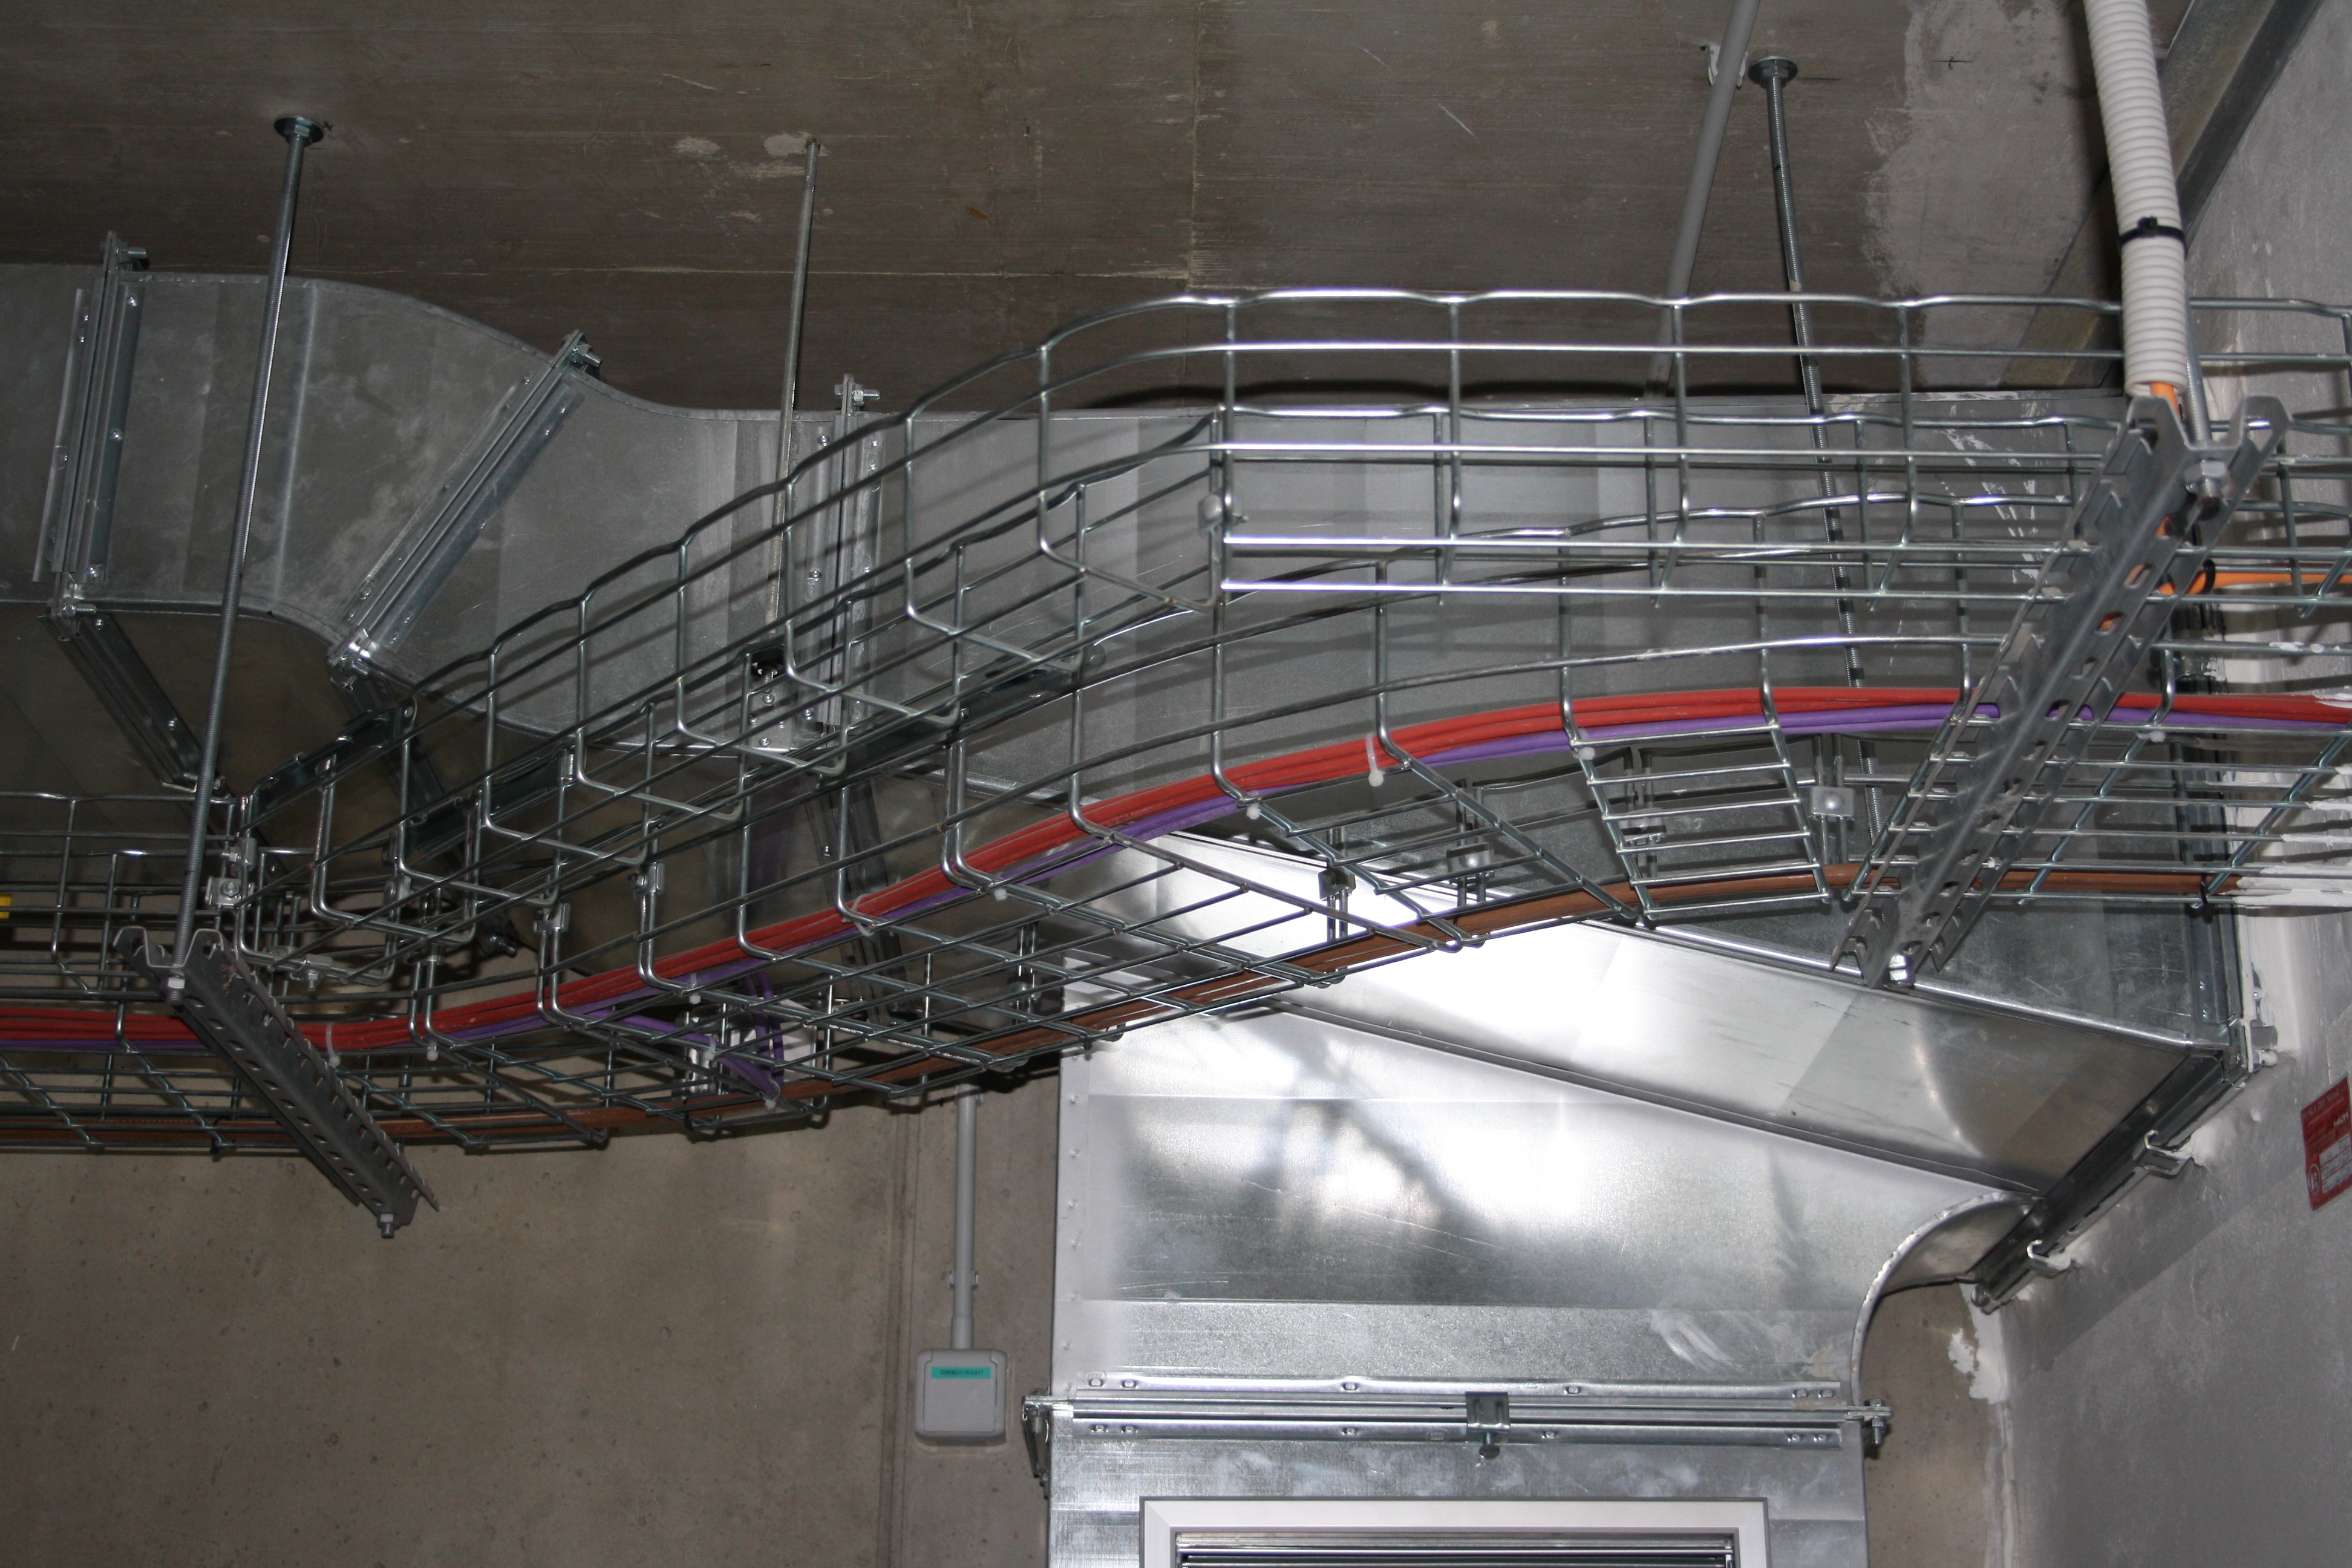
\includegraphics[width=0.47\textwidth]{elektryka/Cabtray_10.jpg} % https://commons.wikimedia.org/wiki/File:Cabtray_10.JPG  Leotard, CC-0
\\
koryta stalowe perforowane i drabiny kablowe &
koryta siatkowe
\end{tabular}\end{center}

\begin{center}\begin{tabular}{ccc}
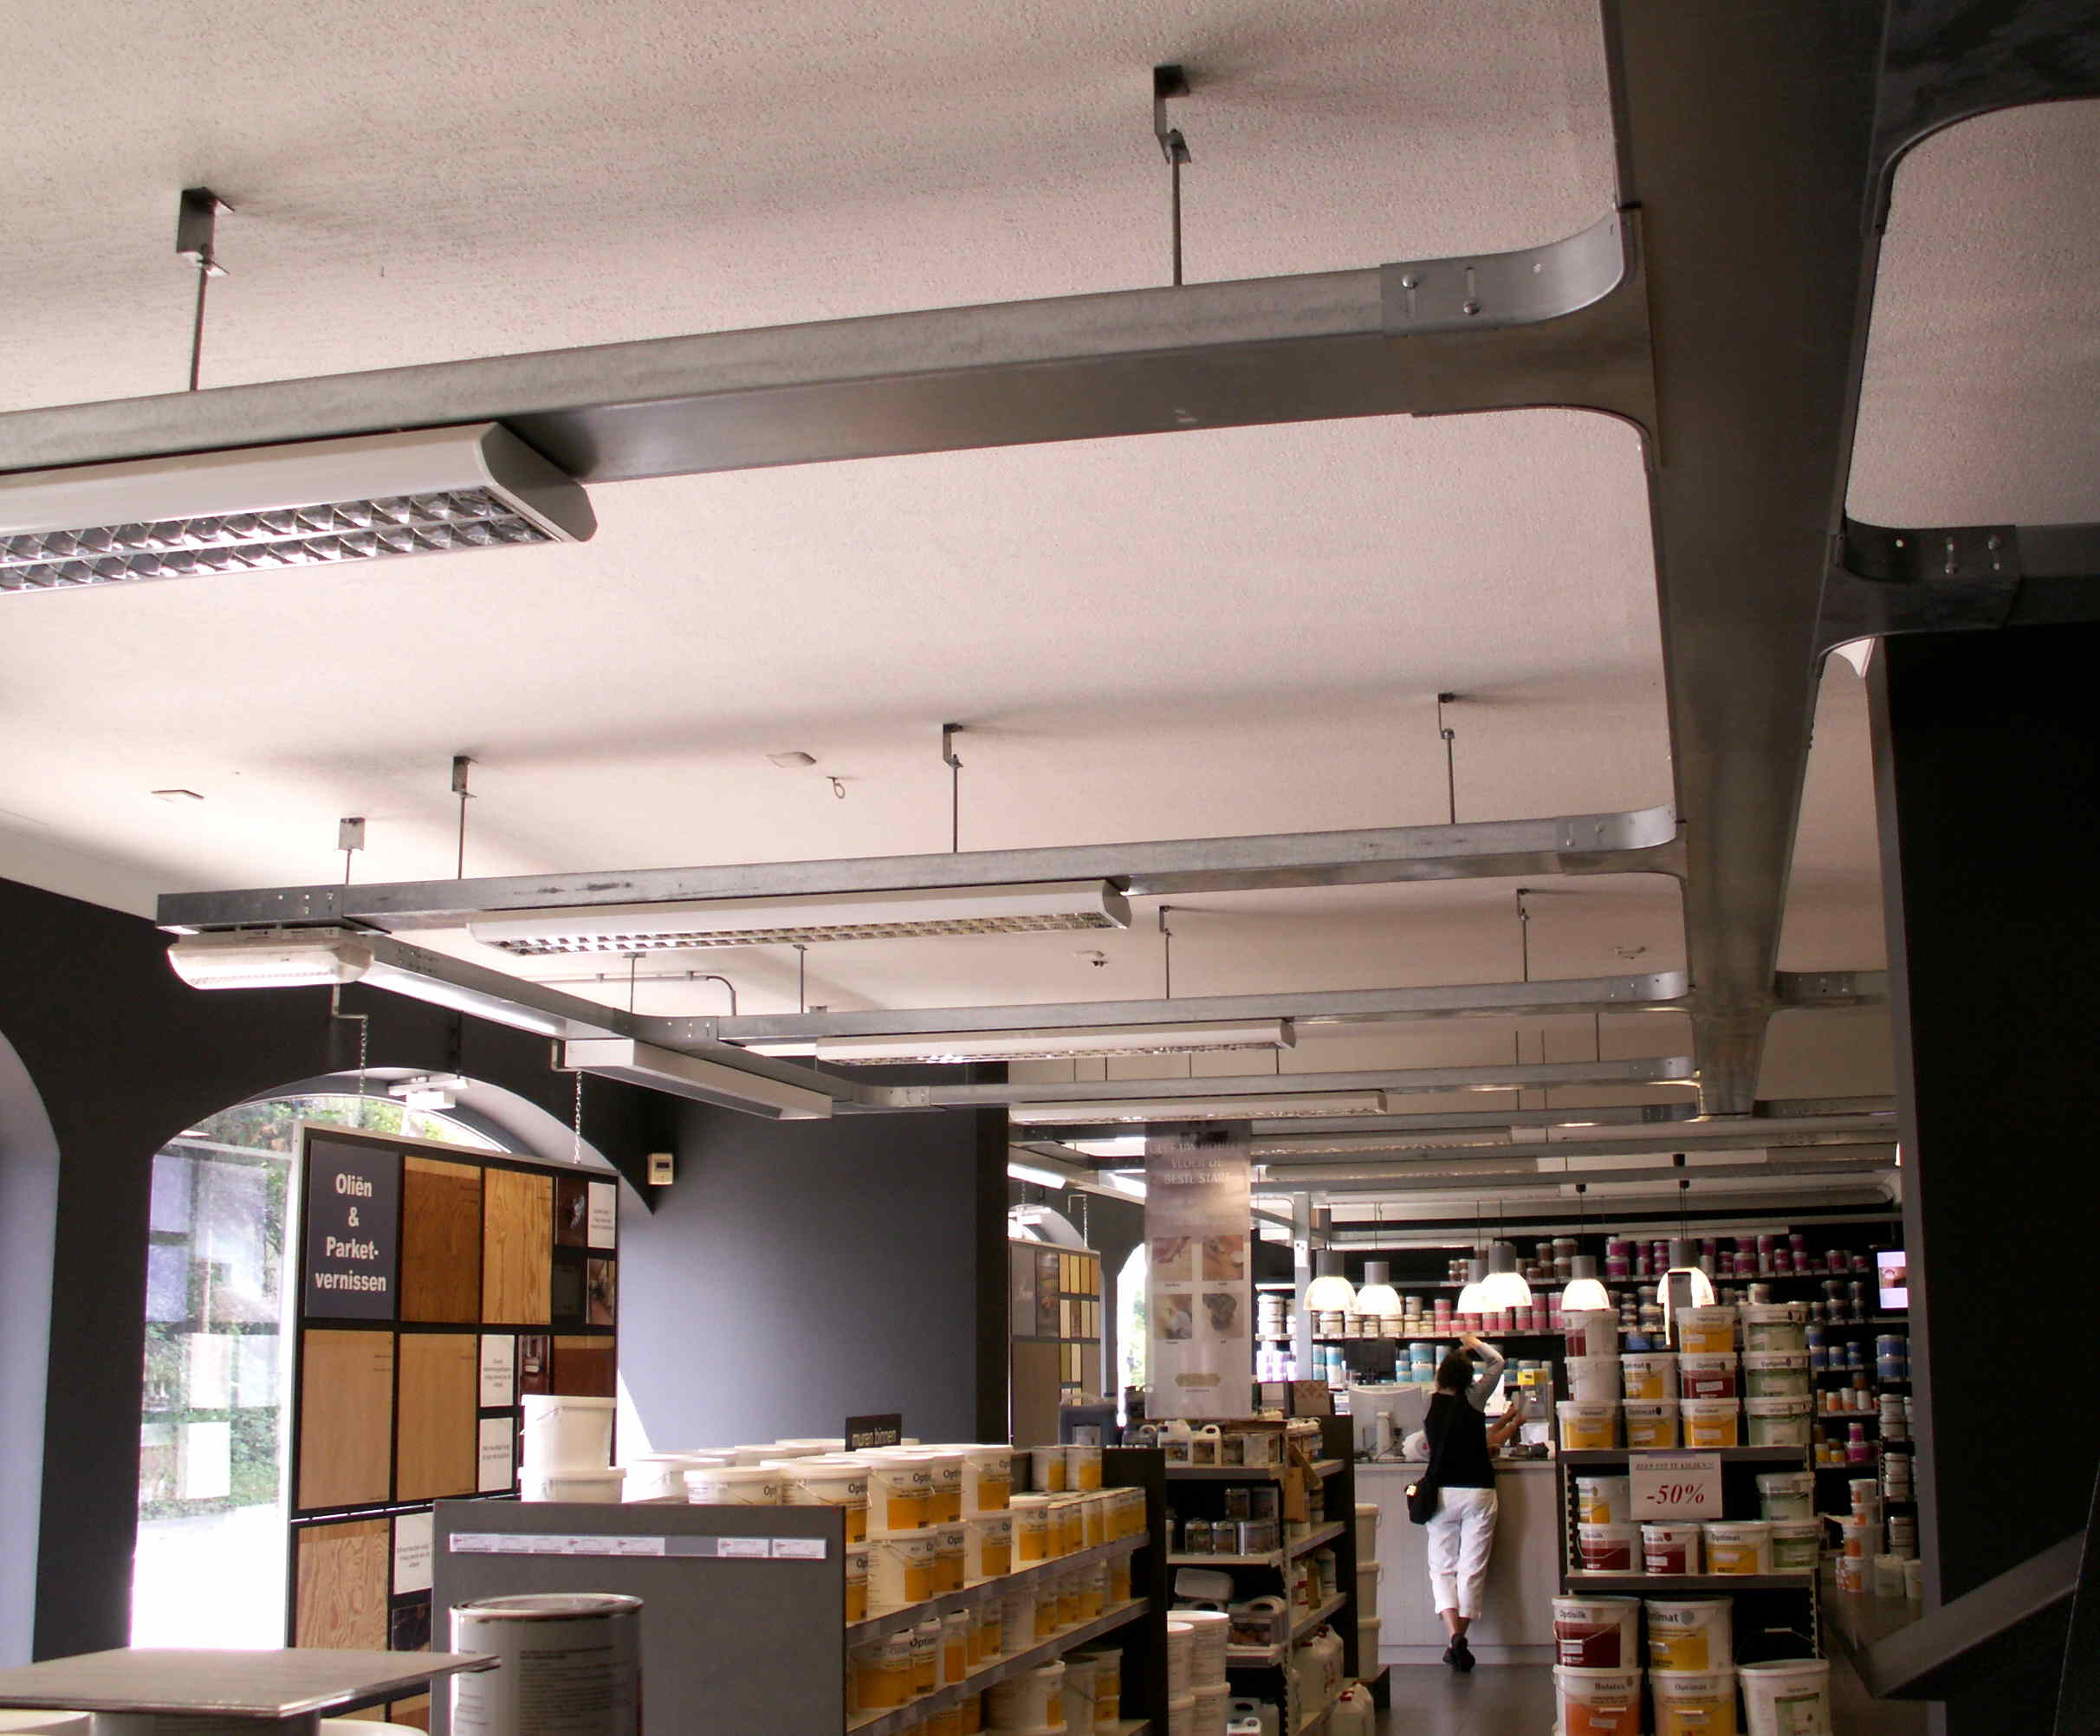
\includegraphics[trim={0 14cm 0 0},clip,width=0.47\textwidth]{elektryka/OrganizedElectricalWiring.jpg} & % https://commons.wikimedia.org/wiki/File:OrganizedElectricalWiring.jpg  KVDP, PD
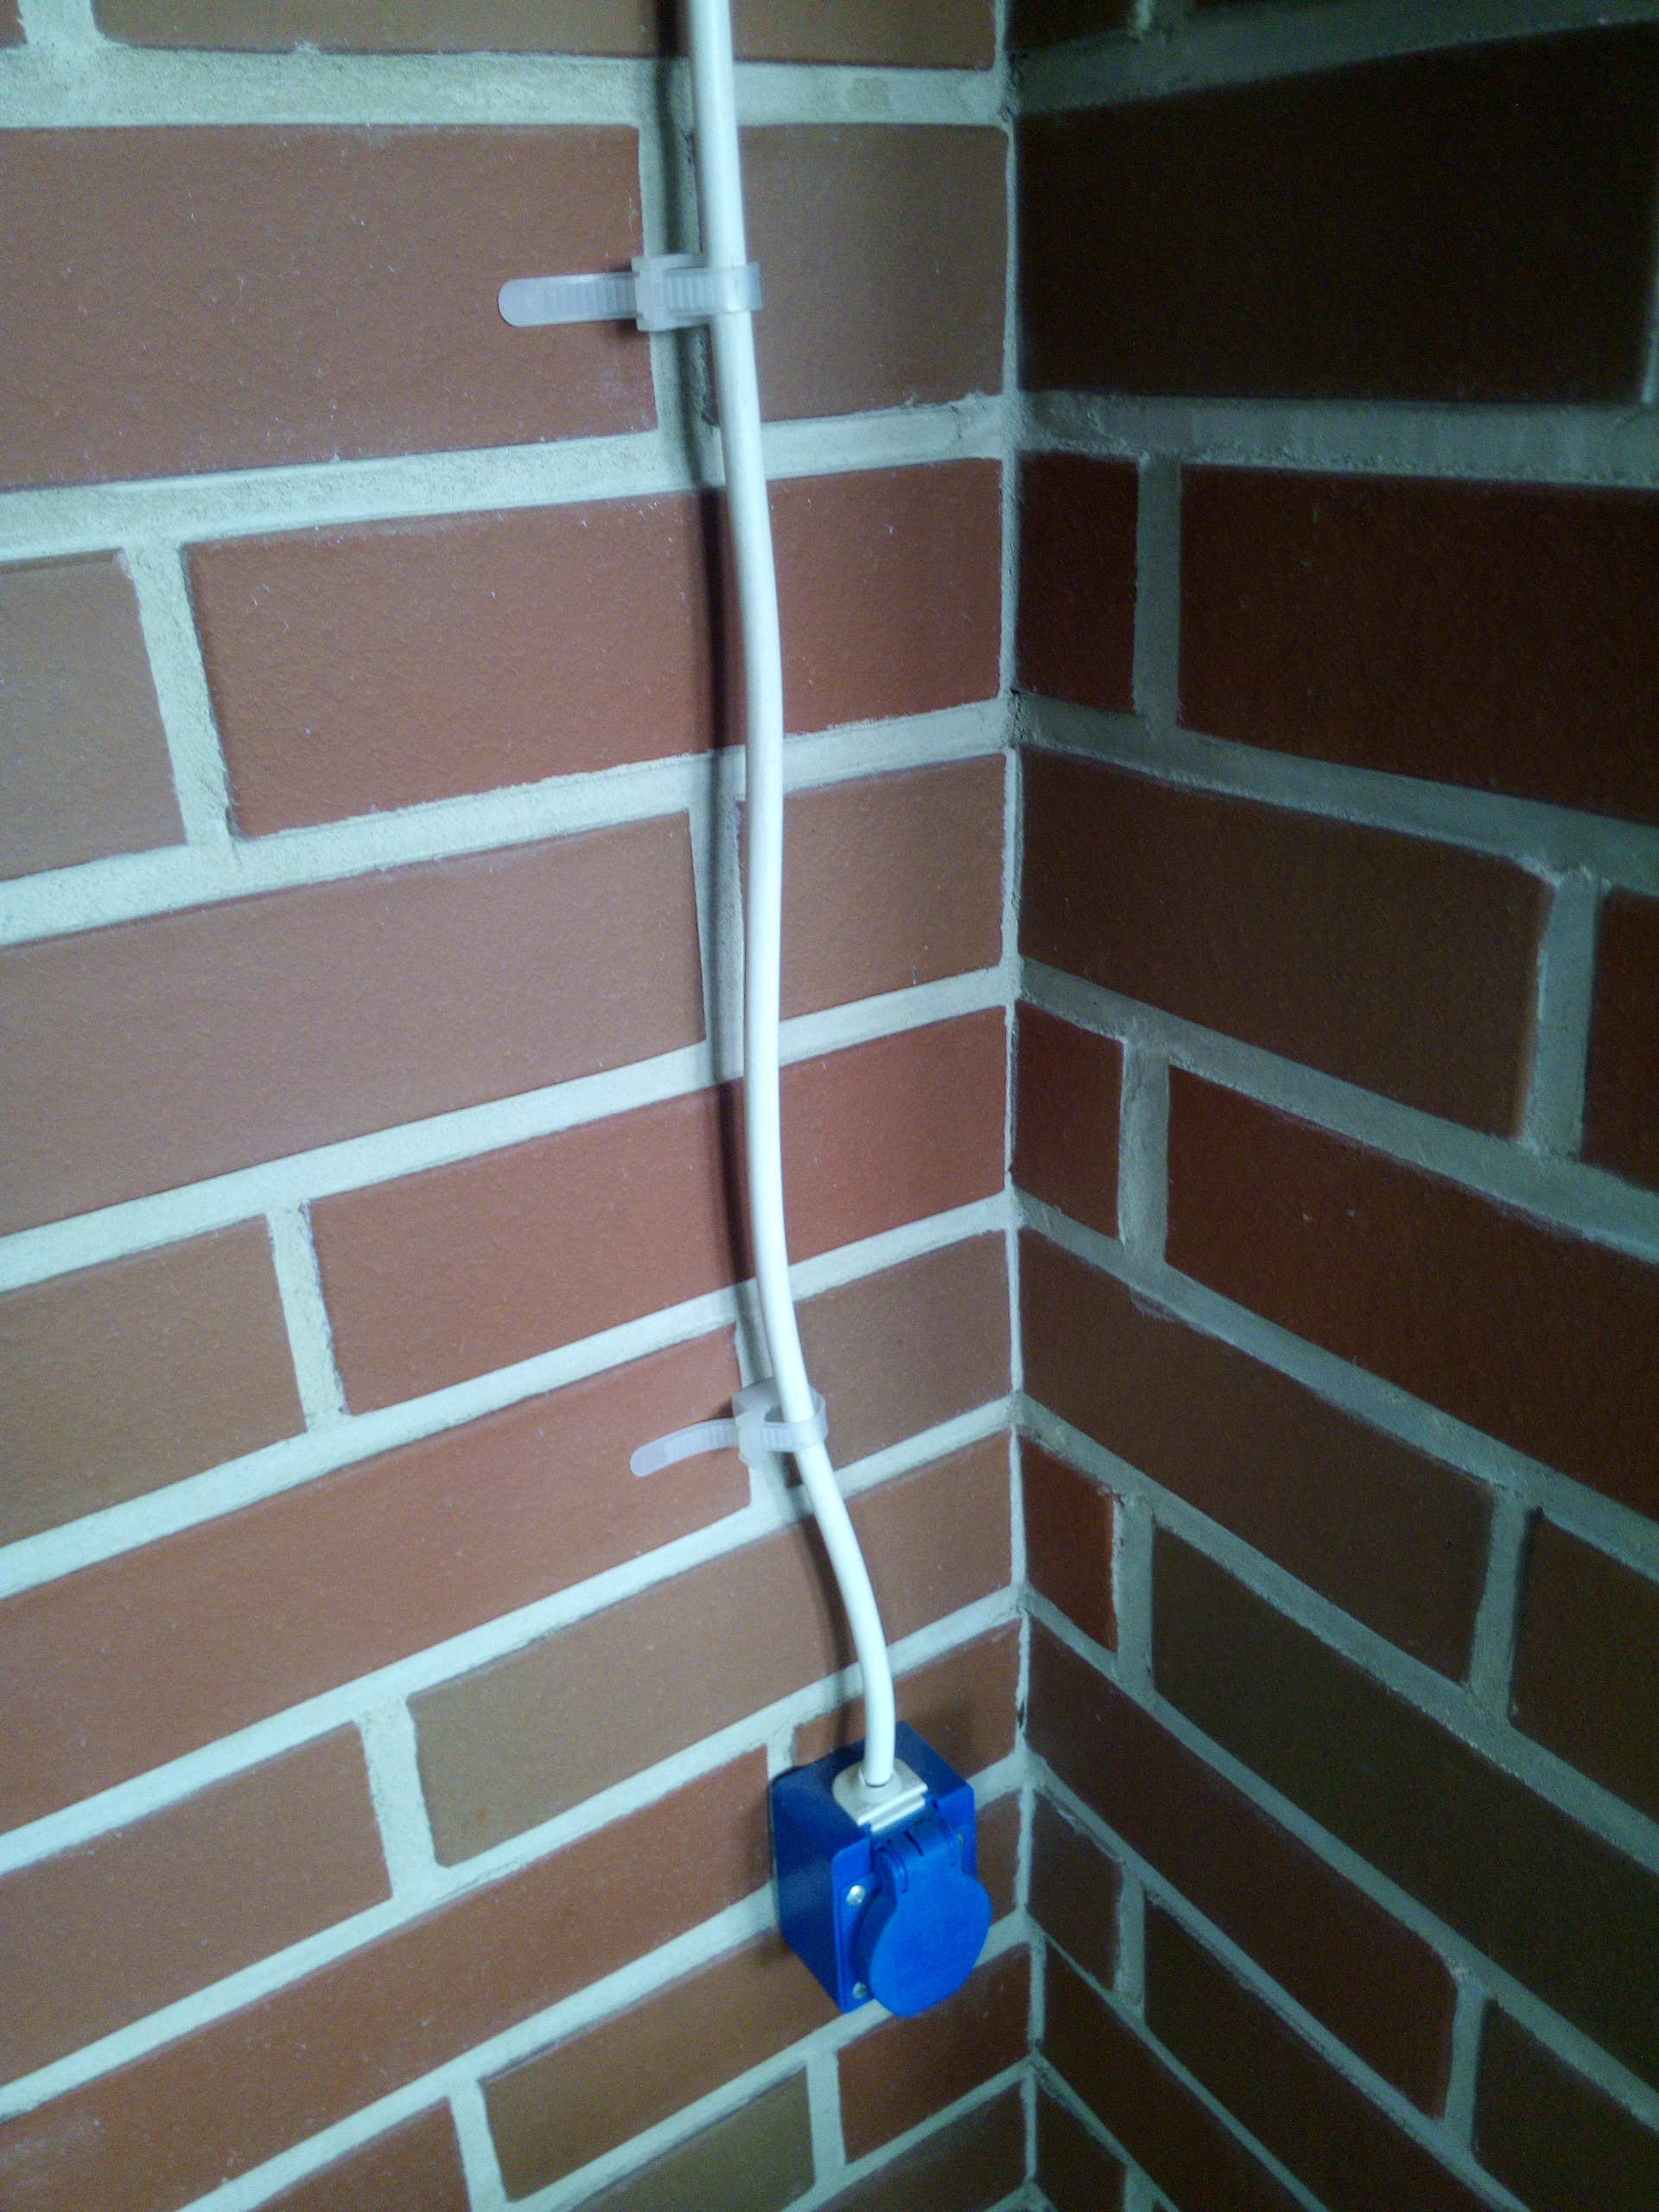
\includegraphics[trim={6cm 0 2cm 0},clip,width=0.176\textwidth]{elektryka/IMG_20210731_145157.jpg} &
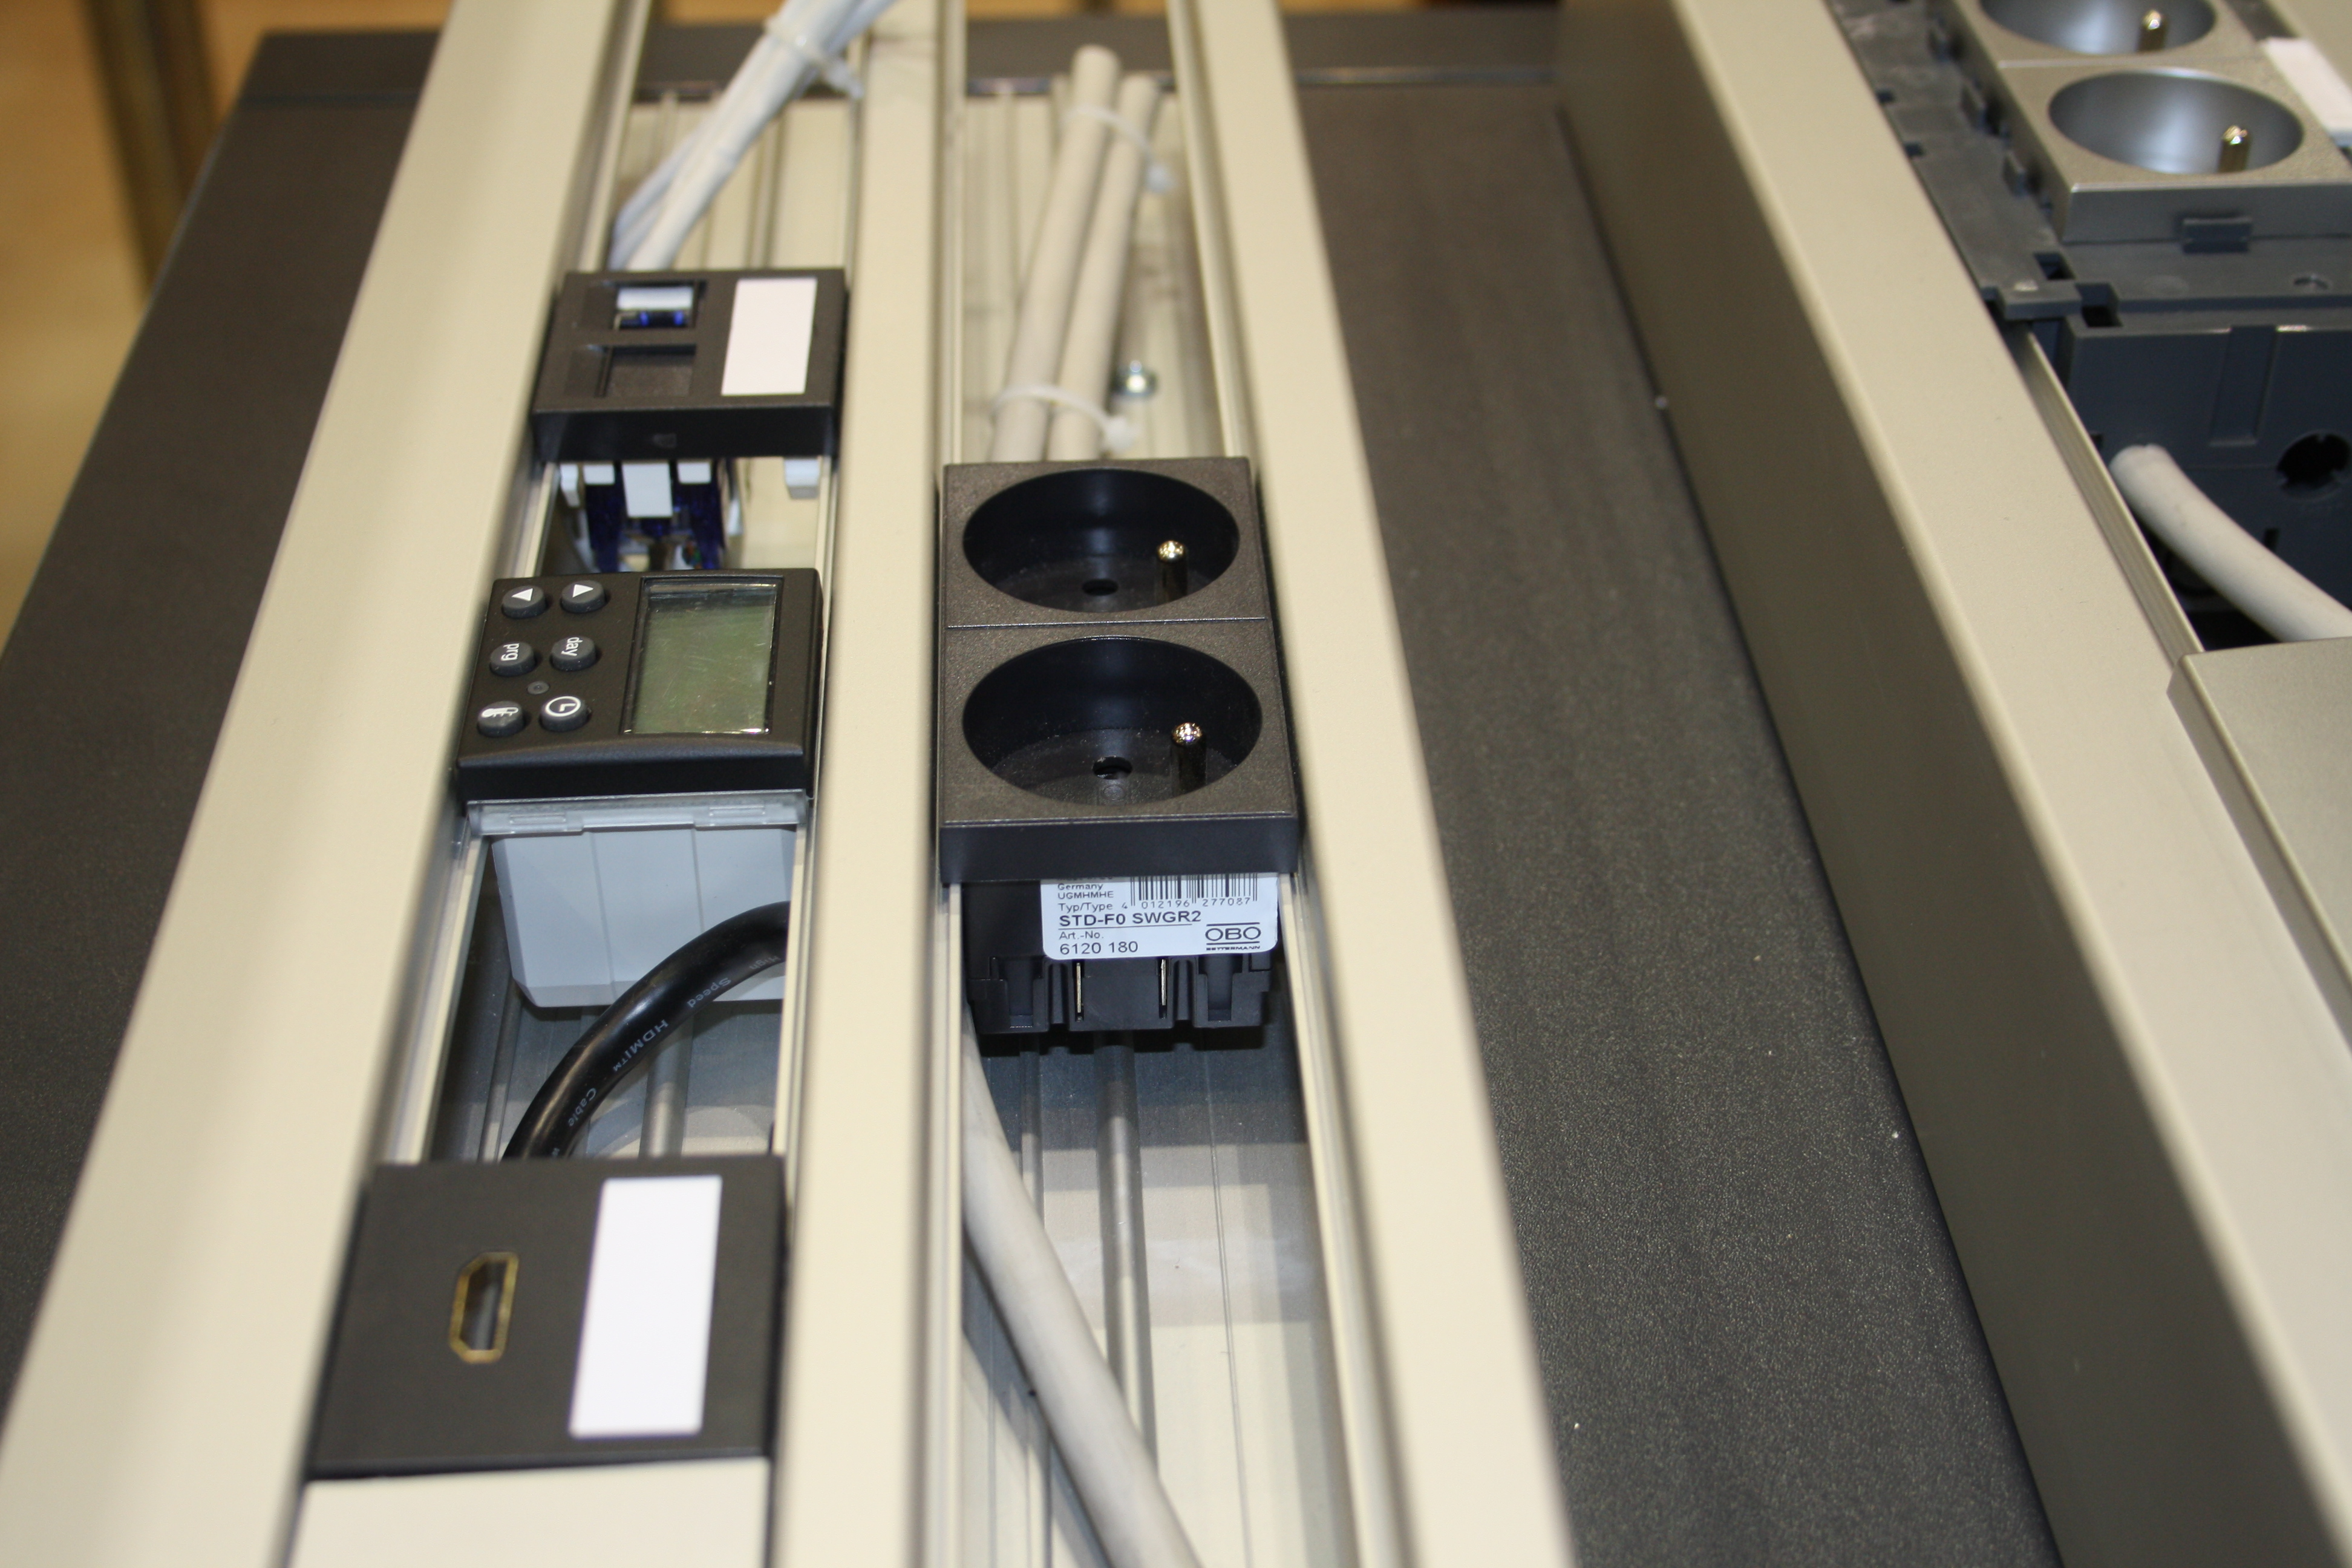
\includegraphics[trim={10cm 0 50cm 0},clip,width=0.263\textwidth]{elektryka/Cabtray_03.jpg} % https://commons.wikimedia.org/wiki/File:Cabtray_03.JPG  Leotard, CC-0
\\
koryta stalowe pełne &
instalacja natynkowa &
kanał instalacyjny PCV
\\
&
bez rurek &
z osprzętem 45x45mm
\end{tabular}\end{center}

\begin{center}\begin{tabular}{cc}
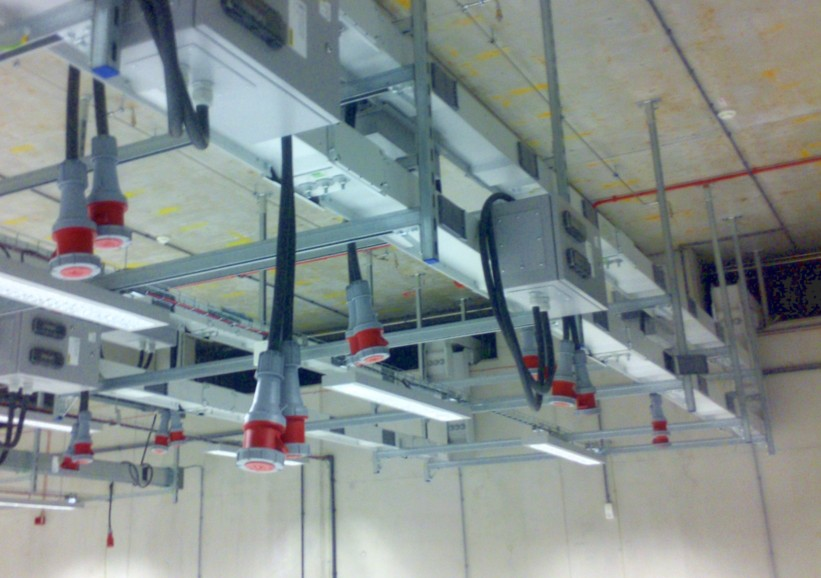
\includegraphics[width=0.47\textwidth]{elektryka/szynoprzewody.jpg} &
\\
szynoprzewody z kasetami dystrybucyjnymi &
\\
powieszone na konstrukcji z ceowników montażowych &
\end{tabular}\end{center}
\end{figure}

\subsubsection{montaż tras kablowych}

Elementy budujące „natynkowe” trasy kablowe, takie jak rurki, czy koryta mogą być montowane bezpośrednio do ściany.
Często jednak stosuje się dodatkowe konstrukcje służące ich zamocowaniu – zwłaszcza w przypadku koryt metalowych i szynoprzewodów.
Pozwalają one na montaż koryta do ściany lub sufitu z zachowaniem „orientacji” koryta w przestrzeni,
	czyli bez jego obracania, tak aby kable leżały na jego dnie a nie boku (dzięki czemu nie będą wypadać i nie ma potrzeby stosowania np. pokrywy do koryta).
Koryta mogą być mocowane do ścian przy użyciu różnego rodzaju wsporników, podwieszane do sufitu za pomocą szpilek,
	czy też montowane zarówno do ścian jak i sufitów na bardziej rozbudowanych konstrukcjach głównie z ceowników montażowych\footnote{
		Ceownik montażowy jest to profil (zazwyczaj stalowy) przypominający w przekroju literę C / U, gdzie boczne ścianki sa lekko zagięte do środka.
		Takie ukształtowanie zapewnia większą sztywność oraz pozwala na montaż elementów do „wnętrza” ceownika z użyciem nakrętek rombowych.
	}.
Zaletą zastosowania konstrukcji z ceowników w stosunku co do podwieszenia na szpilkach jest zapewnienie większej sztywności całej trasie kablowej.
Jest to szczególnie istotne przy montażu szynoprzewodów, które będą obciążane jeszcze dodatkowo skrzynkami odpływowymi –
	zwykłe ich podwieszenie na szpilach nie zapewni sztywności i pozornie sztywne szynoprzeody zaczną się skręcać i chwiać.

\begin{figure}[ht!]
\begin{center}\begin{tabular}{ccc}
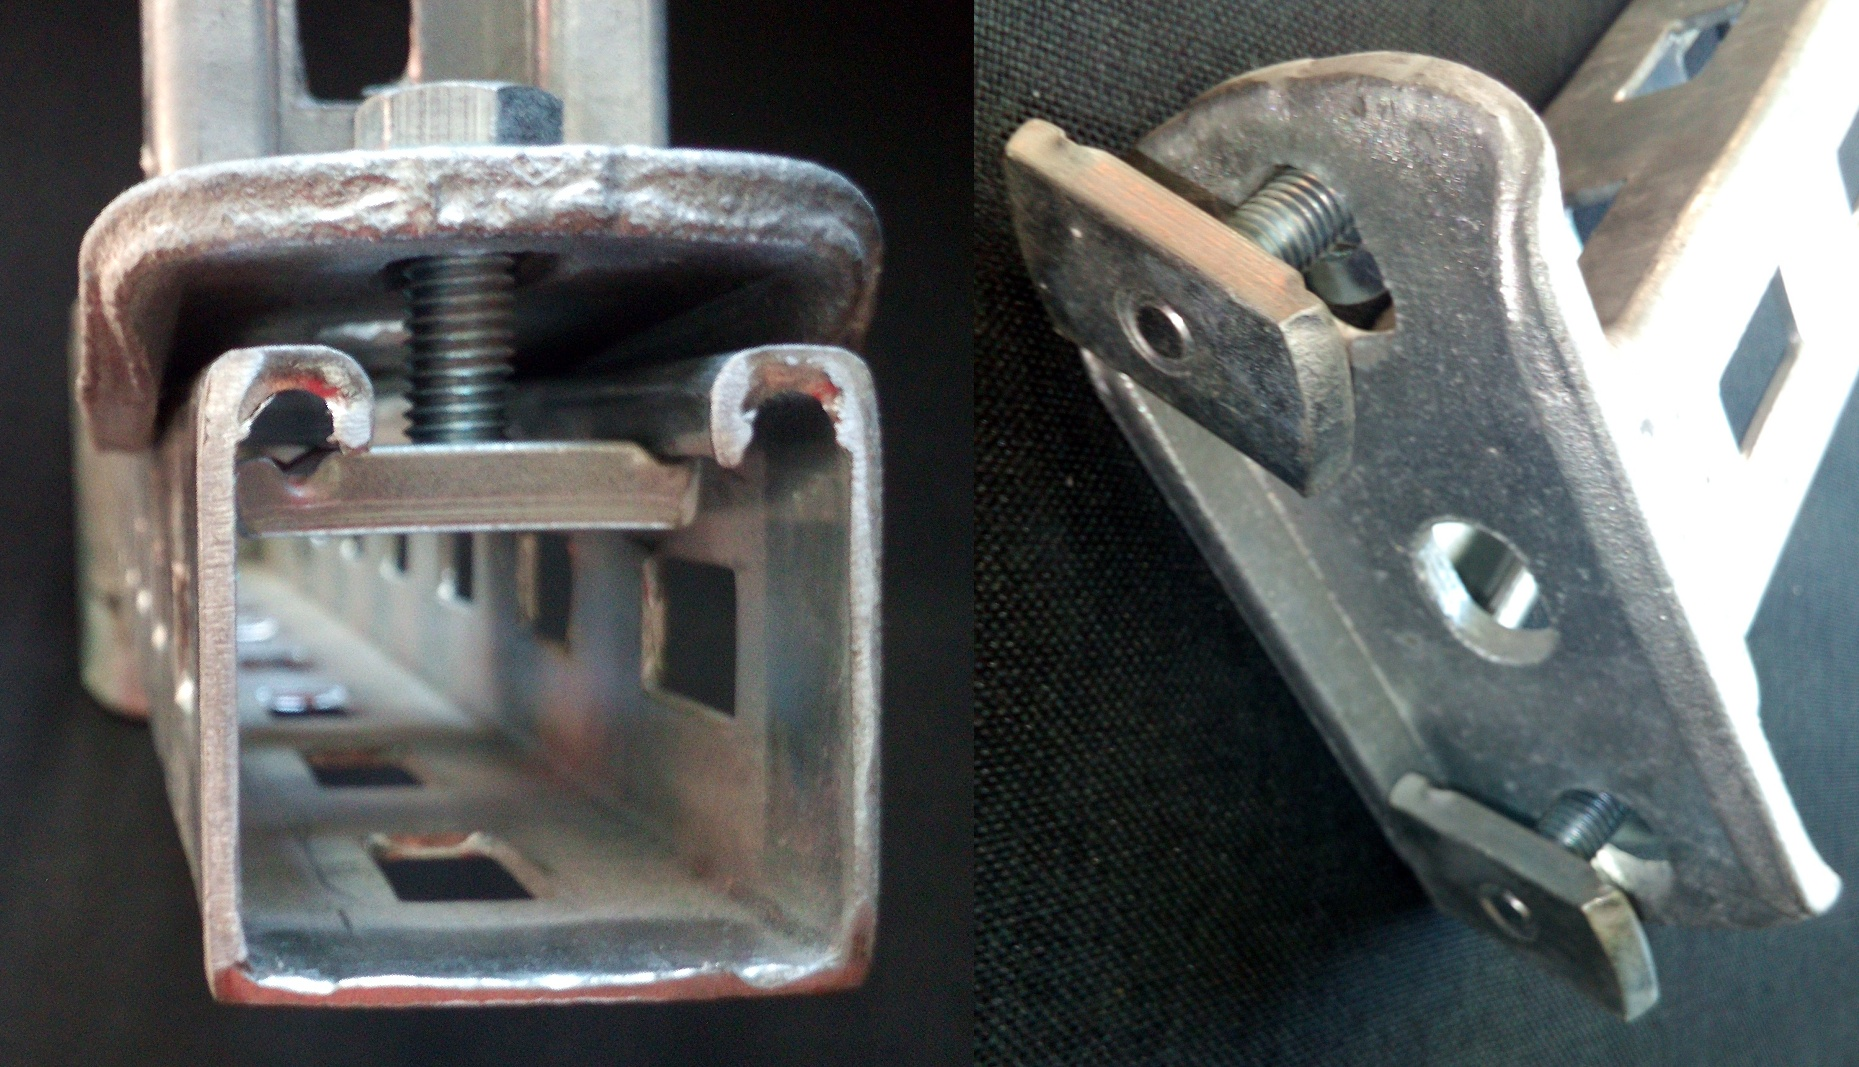
\includegraphics[height=5.5cm]{elektryka/ceowniki1.jpg} &
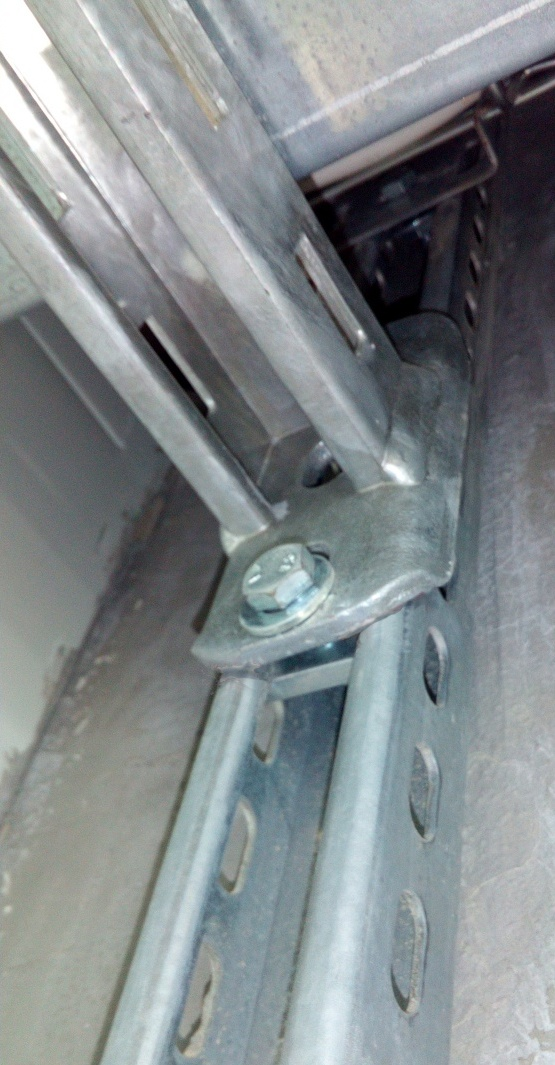
\includegraphics[height=5.5cm]{elektryka/ceowniki2.jpg} &
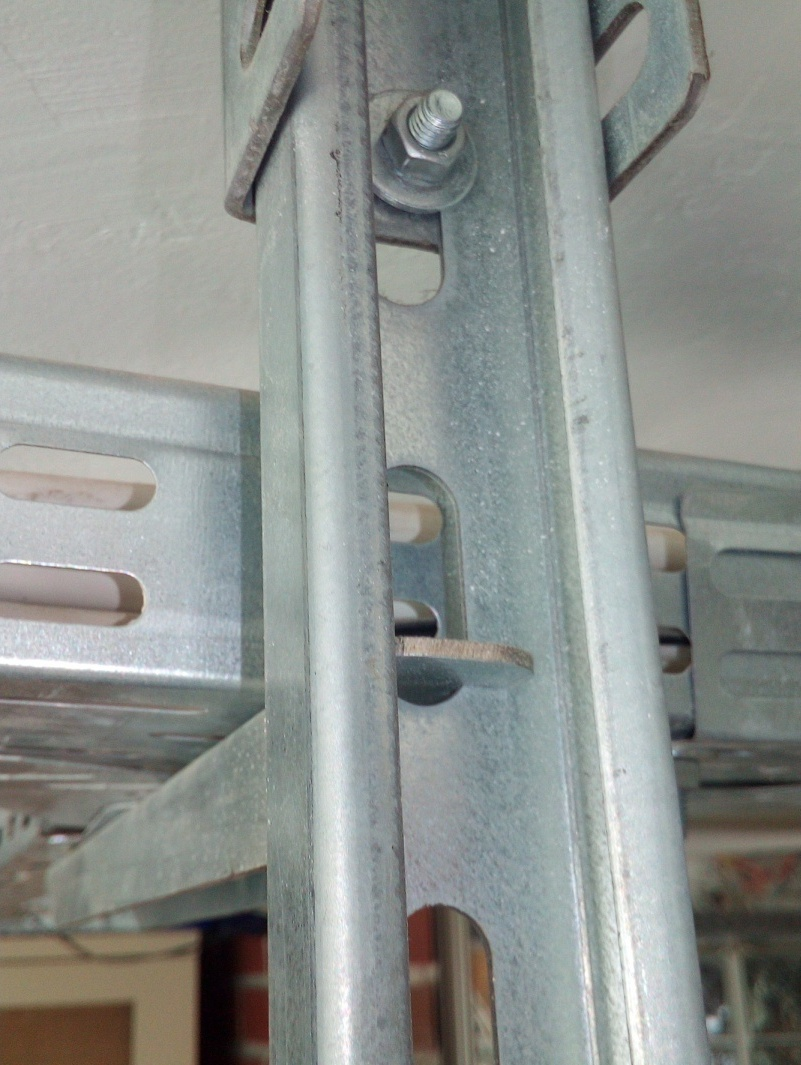
\includegraphics[height=5.5cm]{elektryka/ceowniki3.jpg}
\\
ceownik montażowy wraz z elementem &
wspornik zamocowany &
wykorzystanie perforacji 
\\
montowanym z użyciem nakrętki rombowej &
do ceownika &
ceownika do montażu
\end{tabular}\end{center}
\end{figure}

\subsection{rozdzielnice}

Przy planowaniu, projektowaniu rozdzielnic najistotniejsze jest zapewnienie odpowiednio dużo miejsca w rozdzielnicy – zarówno dla zmieszczenia samej aparatury i okablowania, jak też komfortu wykonywania prac serwisowych (dostęp do wszystkich elementów, zacisków, itd) oraz ew. rozbudowy czy modyfikacji. Przy wykonywaniu (prefabrykacji, montażu, kablowaniu) rozdzielnicy istotna jest estetyka i przejrzystość, która ułatwia późniejsze prace serwisowe.

Istnieje wiele rozwiązań konstrukcyjnych dla rozdzielnic elektrycznych, często nawet pojedynczy producent posiada kilka (niekompatybilnych ze sobą) takich systemów.
Konkretne rozwiązanie konstrukcyjne powinno być dobrane z uwzględnieniem tego co w danej rozdzielnicy będzie się znajdować i jak jest to montowane (szyna DIN, płyta montażowa, rack 19", ...).
Warto jednak pamiętać że na ogół nie wszystko musi się znaleźć w jednej obudowie i czasami lepiej jest zastosować osobną rozdzielnicę modułową i np. osobną obudowę z płytą montażową na pojedynczy duży aparat.
Albo osobną rozdzielnicę elektryczną i osobną szafkę rack na montaż kilku paneli krosowych i switcha.
Istotne jest dobre wykorzystanie miejsca i wykonanie zapewniające wygodę obsługi i serwisu.
Warto aby rozdzielnica zapewniała odpowiednią głębokość, ale raczej należy unikać montażu na kilku głębokościach na tej samej wysokości (pozwala to zmieścić więcej urządzeń, ale utrudnia dostęp).

\subsection{standardy}

\subsubsection{szyna DIN}

\begin{wrapfigure}{r}{2.7cm} %
\vspace{-0.8cm}\includegraphics[trim={0cm 0 0.2cm 0},clip,width=2.5cm]{img/elektryka/DIN-rail-dimensions}\vspace{-0.5cm} % https://commons.wikimedia.org/wiki/File:DIN-rail-dimensions.svg  Markus Kuhn as Public Domain
\end{wrapfigure}

Standard szyny \href{https://en.wikipedia.org/wiki/DIN_rail}{montażowej DIN} określa kilka rodzajów szyn.
Najpopularniejszą z nich jest szyna TH-35, szyli szyna o szerokości 35mm z blachy o grubości 1mm, zagłębiona w środkowej części na szerokości 25mm o co 7.5 mm lub 15mm (zależnie od wariantu).

Sam standard szyny nie określa niczego więcej.
W ogólności kształt obudów montowanych na szynę DIN nie jest zestandaryzowany (spotykane sa np. obudowy o wysokości kilkunastu cm).

Natomiast jest określony kształt obudów aparatury modułowej montowanej na szynę DIN.
Typowy moduł nie przekracza 47mm głębokości od szyny TH do części zakrywanej panelem przednim obudowy, 70mm głębokości od szyny TH do frontu aparatu, który liczy 45 mm wysokości.
Zapewnia to że większość aparatury modułowej da się zainstalować nawet w płytkiej rozdzielnicy bez możliwości regulacji głębokości szyn.
Natomiast szerokość przypadająca na jeden biegun zasilania wynosi 17.5mm, co pozwala na stosowanie standardowych szyn łączeniowych do aparatów.

Typowo długość szyny (szerokość zamontowanych na niej urządzeń) określa się właśnie w modułach o szerokości 17.5mm (±0.5mm).\footnote{Stosowane są także urządzenia o szerokości mniejszej niż jeden moduł – np. styki pomocnicze, złączki kablowe.}
Przez to, że standardowy jednopolowy wyłącznik nadprądowy posiada właśnie szerokość 1 modułu, to ilość modułów daje pewne wyobrażenie o wielkości rozdzielnicy.


\subsubsection{rack 19"}

Standard \href{https://en.wikipedia.org/wiki/19-inch_rack}{rack 19"} wywodzi się z telekomunikacji i jest powszechnie stosowany w rozwiązaniach IT.
Bywa jednak stosowany w zastosowaniach elektrycznych.
Stosowane są moduły wysokości 3U wyposażone w szynę DIN TH-35 do montażu aparatury elektrycznej w ramie rack 19".
Stosowane są także adaptery do montażu (odpowiednio krótkich) urządzeń rack 19" w (dostatecznie szerokich) rozdzielnicach elektrycznych.

Standard rack 19" (\href{https://www.server-racks.com/eia-310.html}{EIA-310}) określa jedynie podstawowe parametry montażowe dla płyt czołowych:
\begin{itemize}
	\item wymiary poziome:
	\begin{itemize}
		\item odległość pomiędzy wewnętrznymi krawędziami szyn montażowych (maksymalną szerokość obudowy montowanego urządzenia): 17~3/4" (450mm)
		\item ogległość pomiędzy środkami otworów montażowych: 18~5/16" (465.1mm)
		\item szerokość płyty czołowej urządzenia obejmującą otwory montażowe: 19" (482.6mm)
	\end{itemize}
\end{itemize}

~\vspace{-32pt}
\begin{wrapfigure}{r}{5.5cm}%
\vspace{-0.4cm}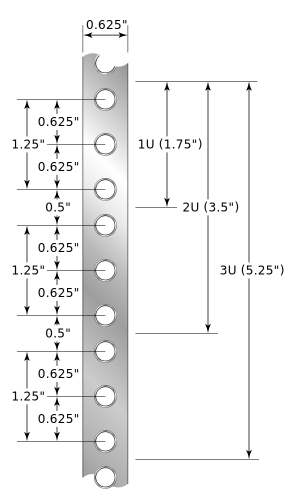
\includegraphics[width=5.3cm]{img/elektryka/Server_rack_rail_dimensions}\vspace{-2.6cm} % https://commons.wikimedia.org/wiki/File:Server_rack_rail_dimensions.svg  Sakurambo as Public Domain
\end{wrapfigure}

\begin{itemize}
	\item wymiary pionowe:
	\begin{itemize}
		\item jednostkę wysokości urządzenia \strong{\href{https://en.wikipedia.org/wiki/Rack_unit}{1U}}=1 3/4" (44.45mm)
		\item odległości środków trzech otworów montażowych w ramach każdego „U”:
			\begin{itemize}
				\item pierwszy otwór: 1/4" (6.35mm) od krawędzi
				\item środkowy otwór: 5/8" (7.95mm) od środka pierwszego
				\item trzeci otwór: 5/8" (7.95mm) od środka środkowego i 1/4" (6.35mm) od krawędzi
			\end{itemize}
			co razem daje 1 3/4" czyli jednostkę wysokości
	\end{itemize}
\end{itemize}

Standard pozwala także na stosowanie różnego typu otworów w profilu montażowym – gwintowane (3/16", 7/32", M5, lub M6), okrągłe niegwintowane lub kwadratowe (3/8" x 3/8", pozwalające na montaż nakrętki typu \textit{\href{https://www.server-racks.com/what-is-a-cagenut.html}{cage nut}}).

Natomiast nie określa:
\begin{itemize}
	\item głębokość szafy ani montowanego sprzętu
	\item formy ani sposobu mocowania jakichkolwiek dodatkowych podparć (dla długich urządzeń), prowadnic kulkowych, itp.
	\item \href{https://www.server-racks.com/rack-upright-shape.html}{kształtu profili} z otworami montażowymi
	\item ilości profili montażowych (czy występują środkowe / tylne)
	\item jakichkolwiek innych aspektów konstrukcyjnych szafy / stojaka (także tego czy to ma być zamknięta szafa czy w pełni otwarty stojak)
\end{itemize}

Można spotkać się także z odmianą 10" oraz 9.5" (half-rack). Ta druga pozwala na montaż dwóch urządzeń obok siebie w standardowym racku 19".
